\documentclass[10pt, letterpaper]{l3doc}

\hypersetup{urlcolor = teal, filecolor = violet}
\hologoFontSetup{general = \sffamily}
\usepackage[mono = false]{libertine}
\usepackage{geometry,framed,xeCJKfntef,enumitem,pdfpages,dirtree}
\setlength{\oddsidemargin}{63pt}\setlength{\evensidemargin}{63pt}
\FrameSep = 0pt 
\usepackage[os = mac]{menukeys}
\AddToHook{env/function/before}{\vspace{-.3\baselineskip}}
\AddToHook{env/syntax/after}{\vspace{-.2\baselineskip}}
\usepackage{datetime}
\yyyymmdddate
\usepackage[fontset = none, scheme = plain]{ctex}
\linespread{1.5}
\setCJKmainfont[AutoFakeSlant]{Songti SC}
\setCJKsansfont[BoldFont = Hei, AutoFakeSlant]{Heiti SC}
\setCJKmonofont[AutoFakeSlant]{LXGW WenKai Mono}
\renewcommand{\emph}[1]{\CJKsout*[thickness=2.5ex, format=\color{blue!15}]{#1}}

\title{\bfseries The \textsc{\cls{HduThesis}} Class\\
\hologo{LaTeX} Thesis Template for Hangzhou Dianzi University}
\author
{
  Mingyu Xia \texttt{<\href{mailto:xiamyphys@gmail.com}{xiamyphys@hdu.edu.cn}>}
  \footnote{
    School of Sciences, Physics Department, Graduate in 06/2025 (expected)
  }
}
\date{v0.2.0\footnote{\url{https://github.com/xiamyphys/hduthesis}} ~(\today)}

\begin{document}

\begin{titlepage}
  \newgeometry{margin = 1in}
  \maketitle
  \begin{center}
    \tikz
    {
      \node [opacity = .8] 
      {
\includegraphics[width = .2\paperwidth]{hdumotto.pdf}};
      \node [opacity = .3]
      {
\includegraphics[width = .3\paperwidth]{hdulogo.pdf}};
    }
  \end{center}
  \begin{abstract}
    \textsc{\pkg{HDUThesis}} 是杭州电子科技大学毕业论文 \hologo{LaTeX}模板,支持学士和硕士学位论文排版.
    \vspace*{1em}
    \begin{center}
      \footnotesize\bfseries User Agreement
    \end{center}
    \begin{enumerate}[leftmargin = 2.5ex]
      \item 本模板通过 LPPL 1.3c 协议开放源代码,您可以随意使用编译出的 PDF 文件.
      \item 本模板根据杭州电子科技大学教务处颁发的 \href{https://jwc.hdu.edu.cn/2022/0428/c4528a153813/page.htm}{杭电理工类毕业论文写作规范} 编写而成. 作者不对使用本模板产生的格式审查问题负责. \emph{如果您所在的学院因论文查重、收录等原因要求提交 \file{.docx} 格式,不接收 \file{.pdf} 论文稿件,请勿执意使用本模板,避免因格式转换带来不必要的麻烦.}
      \item 欢迎前往 GitHub 提交反馈意见,为推动学校认证与规范化 \textsc{\cls{HduThesis}} 贡献力量.
    \end{enumerate}
  \end{abstract}
  \thispagestyle{empty}
\end{titlepage}
\restoregeometry

\section{Generate the Cover}

\begin{function}{\DocInfo}
  \begin{syntax}
    \cs{DocInfo}\marg{keyvals}
  \end{syntax}

  此命令接收键值,用于设置文档信息. 键 \keys{\cmdmac~title} 用于设置论文标题,键 \keys{\cmdmac~school} 用于设置学院,键 \keys{\cmdmac~major} 用于设置专业,键 \keys{\cmdmac~class} 用于设置班级,键 \keys{\cmdmac~stdntid} 用于设置学号,键 \keys{\cmdmac~author} 用于设置作者,键 \keys{\cmdmac~supervisor} 用于设置导师,键 \keys{\cmdmac~reference} 用于设置插入参考文献文件源.

  \begin{framed}
    \begin{verbatim}
    \documentclass { hduthesis }
    \DocInfo
    {
      title      = 杭州电子科技大学学位论文 \hologo{LaTeX} 模板/
                   \hologo{LaTeX} Template for Thesis at Hangzhou Dianzi University,
      school     = 理学院,                   major     = 物理学,
      stdntid    = C668668E00,               author    = 申智能/SAN Chi Nan,
      supervisor = 李智能/LEE Chi Nan,       reference = reference
    }
    \begin{document}  \maketitle  ...  \end{document}
    \end{verbatim}
  \end{framed}

  命令会根据输入的学号自动判断使用者为本科生/研究生 \footnote{杭州电子科技大学本科生学号为8位,研究生学号为10位.}. 依学校要求,硕士学位论文扉页需同时有英文版. 因此需要在键 \keys{\cmdmac~title} \keys{\cmdmac~author} \keys{\cmdmac~supervisor} 中输入中文和英文信息. 如作者中文姓名为 \cmd{申智能},英文姓名为 \cmd{SAN Chi Nan},则键值输入格式为 \cmd{author = 申智能/SAN Chi Nan}.

  对于本科生,则需要使用键 \keys{\cmdmac~title} 设置类型为毕业设计/毕业论文,即 \cmd{title = Title/毕业设计}.

  命令 \cs{DocInfo} 需在导言区中执行. 通过此命令完成文档信息输入后,在 \verb|\begin{document}| 后执行命令 \cs{maketitle} 会调用所设置的键值并自动生成 \emph{论文封面} 和 \emph{诚信承诺书}.
\end{function}

\begin{function}{\l__hduthesis_grade_int}
  \begin{syntax}
    \cs{ExplSyntaxOn}  \cs{int_set:Nn} \cs{l__hduthesis_grade_int} \marg{Year}  \cs{ExplSyntaxOff}
  \end{syntax}

  论文完成日期和学生毕业年份会根据当前系统时间自动生成. 如果当前月份在8月及以前,毕业年份会显示当前年;如果当前月份在9月及以后,毕业年份会显示次年. 

  在导言区 \cs{DocInfo} 命令后对整型 \cs{l__hduthesis_grade_int} 重新赋值可强制更改毕业年份.
\end{function}

下页包含所生成的本科毕业设计与硕士学位论文封面、扉页和承诺书缩略图. 本科毕业设计与硕士学位论文样例可分别在终端执行 \cmd{texdoc hduthesis-bc} 和 \cmd{texdoc hduthesis-pg} 获取.

文档类同时提供了校徽 (\file{hdulogo.pdf})、校牌 (\file{hdubadge.pd}) 与校训 (\file{hdumotto.pdf}) 的矢量素材,可直接使用. 以上文件均由 \href{https://www.hdu.edu.cn/666/list.htm}{校情纵览/校标规范} 所提供素材裁切制成,均支持在 \hologo{XeLaTeX} 和 \hologo{pdfLaTeX} 编译器下使用 \pkg{tikz} 等方式设置透明度.

\section{Enter Abstract in EN / CN}

\begin{function}{abstract (env.),\keywords}
  \begin{syntax}
    \cs{begin}\{abstract\}[en]  ...\cs{keywords}\marg{keywords list}  \cs{end}\{abstract\}
    \cs{begin}\{abstract\}[cn]  ...\cs{keywords}\marg{关键词列表}      \cs{end}\{abstract\}
  \end{syntax}

  环境 \env{abstract} 用于生成摘要,其可选参数可设置语言格式. 命令 \cs{keywords} 需在 \env{abstract} 环境内执行,其会根据 \env{abstract} 环境所选择的语言,自动生成英文 / 中文格式的关键词.
  
  通过命令 \cs{keywords} 以半角逗号 (,) 为分隔输入关键词列表,输出时会根据所处 \env{abstract} 环境选择的语言不同,自动以半 / 全角分号分隔.
  
  \begin{center}
    \fbox{\includegraphics[page = 3, width = .47\linewidth]{hduthesis-bc}}
    \hfill
    \fbox{\includegraphics[page = 4, width = .47\linewidth]{hduthesis-bc}}
  \end{center}
\end{function}

\includepdfmerge
  [
    angle = -90, nup = 2x3, frame, linktodoc, scale=0.94,
    delta = \fpeval{(11-1.5*8.5*210/297)/8}1in
            \fpeval{(11-1.5*8.5*210/297)/3}1in
  ]
  { hduthesis-pg, 2, hduthesis-bc, 1, hduthesis-pg, 3,
    hduthesis-bc, 2, hduthesis-pg, 4, hduthesis-pg, 1
  }

\section{Input Text}

\textsc{\cls{HduThesis}} 的 {chapter}、\cs{section}、\cs{subsection}、\cs{enumerate} 等段落级次均已按``\href{https://jwc.hdu.edu.cn/2022/0428/c4528a153813/page.htm}{杭电理工类毕业论文写作规范}''定制,可直接使用.

如需插入参考文献,通过命令 \cs{DocInfo} 导入 \file{.bib} 文件后在文章末尾输入 \cs{printbiblography} 即可输出参考文献列表. 文档已将参考文献格式设置为 \cmd{gb7714-2015}. 若未指定参考文献 \file{.bib} 文件,为加速编译,\pkg{gbt7714} 宏包将不会加载. 同时,模板额外预置了以下宏包

\begin{table}[htbp]
  \centering
  \begin{tabular}{*{8}{p{.096\linewidth}}}
    \toprule
    \pkg{amsmath}    & \pkg{amssymb}   & \pkg{bm}         & \pkg{booktabs} &
    \pkg{cancel}     & \pkg{circuitikz}& \pkg{cleveref}   & \pkg{derivative} \\
    \midrule
    \pkg{extarrows}  & \pkg{fixdif}    & \pkg{listings}   & \pkg{mathtools}  & \pkg{multicol}   & \pkg{pgfplots}  & \pkg{physics2}   & \pkg{siunitx}\\
    \bottomrule
  \end{tabular}
\end{table}

\begin{center}
  \fbox{\includegraphics[page = 5, width = .3\linewidth]{hduthesis-bc}}
  \hfill
  \fbox{\includegraphics[page = 11, width = .3\linewidth]{hduthesis-bc}}
  \hfill
  \fbox{\includegraphics[page = 12, width = .3\linewidth]{hduthesis-bc}}
\end{center}

\appendix
\section{模块化设计架构}

\linespread{1.02}
\dirtree{%
.1 ./tex/.
.2 hduthesis.cls.
.3 hduthesis-font-module.code.tex: \footnotesize 字体模块.
.3 hduthesis-unv.layout-module.code.tex: \footnotesize 共用布局模块.
.3 hduthesis-bc.layout-module.code.tex: \footnotesize 本科模块.
.3 hduthesis-pg.layout-module.code.tex: \footnotesize 硕士布局模块.
.3 hduthesis-preamble-module.code.tex: \footnotesize 中英摘要模块.
.2 hdulogo.pdf: \footnotesize 校徽.
.2 hdubadge.pdf: \footnotesize 校牌.
.2 hdumotto.pdf: \footnotesize 校训.
}

\end{document}
